documentclass[class=minimal,border=10pt]{standalone}
\usepackage{tikz}
\usetikzlibrary{matrix,arrows.meta}
\tikzset{
    block/.style = {draw, fill=gray!20, minimum width=3cm, minimum height=2cm},
    input/.style = {draw, fill=gray!20, minimum width=5cm, minimum height=2cm},
    blockchannel/.style = {draw, fill=gray!20, minimum width=3cm, minimum height=1.7cm},
    blocktransformer/.style = {draw, fill=gray!20, minimum width=3cm, minimum height=2cm},
    line/.style = {-Triangle},
    arrow/.style = {-Triangle,dashed},
    annot/.style = {align=center},
    }
\begin{document}
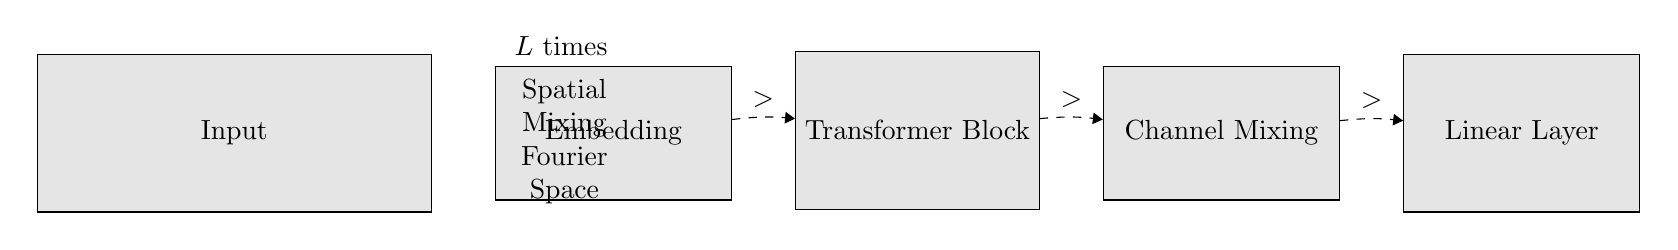
\begin{tikzpicture}[auto]
    % Define blocks for each image
    \matrix (m) [matrix of nodes,row sep=8mm,column sep=8mm,minimum width=2cm]
    {
        \node [input] (input) {Input}; & \node [blockchannel] (embedding) {Embedding}; & \node [blocktransformer] (transformer_block) {Transformer Block}; & \node [blockchannel] (channel_mixing) {Channel Mixing}; & \node [block] (linear_layer) {Linear Layer}; \\
    };
    \path [line] (input) -- (embedding);
    \path [arrow] ([shift={(-0.6,0)}]embedding.north east) --++ (right:0.8) |- ([shift={(0,-0.4)}]embedding.north west) coordinate[pos=0.9] (tmp) -| ([shift={(0.4,0)}]embedding.south east);
    \path [arrow] (tmp|-embedding.north east) --++ (right:0.2) node [above] (tmp) [align=center] {$L$ times};
    \path [arrow] (embedding) edge [bend left=6] node [annot,midway,above,sloped] (tmp) {$>$} (transformer_block);
    \path [arrow] (transformer_block) edge [bend left=6] node [annot,midway,above,sloped] {$>$} (channel_mixing);
    \path [arrow] (channel_mixing) edge [bend left=6] node [annot,midway,above,sloped] {$>$} (linear_layer);
    \node [annot,anchor=north west] at (embedding.north west) {\begin{tabular}{c}Spatial \\Mixing \\ Fourier \\ Space\end{tabular}};
    \end{tikzpicture}
\end{document}